\section{Discussion}
\label{sec:discussion}

\subsection{What was searched}
\label{sec:newspace}

The search space opened here is millimetre and submillimetre frequency toward
the nearest stars: \CvUnionA\,GHz between \SurvFreqLoA{} and
\SurvFreqHiA\,GHz toward systems within 40\,pc, where the only other search
of more than a single line covered \MasonBandMHz\,MHz of Band~3
(\S\ref{sec:intro}). The channels were inherited, not chosen: from
\SzChanFinestKHz\,kHz to \SzChanWidestMHz\,MHz, against the \SzChanLitHz\,Hz
of centimetre-band carrier searches (Fig.~\ref{fig:context}(b)).

Union bandwidth overstates what that buys, because frequencies were searched
toward different stars to very different limits. Figure~\ref{fig:covmap}
therefore counts the systems in which a carrier of a
given EIRP and sky frequency would have been recovered nine times in ten. At
$\CovEirpRefTex$\,W the covered frequency falls to \CovUnionAtRef\,GHz,
\CovFracAtRef{} per cent of the union, and reaches \CovNSysAtRef{} systems,
\CovNMaxAtRef{} of them near \CovNuMaxAtRef\,GHz. At any power that frequency
reaches \CovNMaxFull{} of the \NSysClassA{} systems, and half the sample is
reached only above $\CovEirpHalf$\,W.

\begin{figure}
\centering
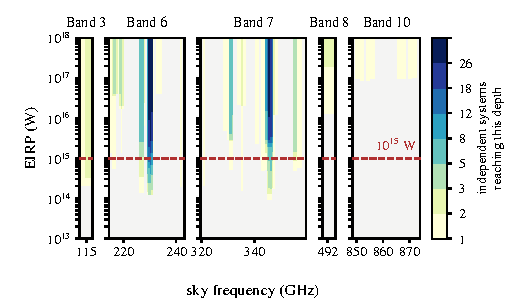
\includegraphics[width=\columnwidth]{figures/completeness_map.pdf}
\caption{Where the experiment could have found something. Shading, the
independent systems recovering an unresolved carrier of the plotted EIRP and
sky frequency nine times in ten \emph{in a single epoch}; unshaded, none.
Confirmation needs a second epoch covering the same frequency, which no
power supplies. Panels as in Fig.~\ref{fig:waterfall}b, which gives that coverage.
Dashed, $\CovEirpRefTex$\,W.}
\label{fig:covmap}
\end{figure}

\subsection{What the non-detection constrains}
\label{sec:excludes}

Every limit here applies to one kind of signal: an unresolved carrier at the
stellar position, confined to a single \ChanLoA--\ChanHiA\,kHz channel, lying
outside the molecular-line mask, radiating while an archival block was on sky,
and drifting linearly within its window's ceiling of
\DriftCeilLo--\DriftCeilHi\,nHz. That covers every known planet of the sample
except \AccelWorstName, reached only as precisely as its host's mass and orbit
are known (\S\ref{sec:statistic}); a transmitter on a rapidly rotating planet
spends most of it on spin (Fig.~\ref{fig:accel}). Emission broader than a channel needs close to
\ScNBroadRatio$\times$ the power for a feature as wide as the widest line in
these fields, and a carrier on for part of a block is recovered at that
fraction of its amplitude. Nothing is constrained inside the
$\pm\MaskHalfKms$\,km\,s$^{-1}$ mask, or toward the stars within 40\,pc that
ALMA has not observed, almost all of the \NGaiaCensus{} this volume holds. The
result is therefore a non-detection, not an exclusion of persistent
transmitters, for the reasons of \S\ref{sec:mmdifferent}.

\noindent\emph{Two blind spots.} The analysis forms
$(\mathrm{XX}+\mathrm{YY})/2$, which retains the full intensity of a circularly
polarised carrier. The loss is not sensitivity but the discrimination
polarisation would offer against unpolarised astrophysical emission: ALMA's
feeds are linear, and the circularity lies in the cross-hands, which this
analysis does not extract. And the \SbPriorFreqGHz\,GHz positronium hyperfine
line that \citet{Steffes1994} and \citet{Mauersberger1996} observed lies in
ALMA Band~5, where this survey holds \LnBFiveWin{} coarse-channel windows, all
toward \LnBFiveStars, and none of them covers it.

\subsection{What prevents stronger conclusions}
\label{sec:mmdifferent}

Depth is not the main limit. An illustrative benchmark, a \BenchDiam\,m dish
radiating \BenchPowerMW\,MW at \BenchFreqGHz\,GHz with an aperture efficiency
of \BenchEta, has a directive gain $G=\eta(\pi D\nu/c)^{2}=\BenchGain$ and so
an EIRP of $\BenchEirp$\,W, above the single-epoch limit of \BenchNSysA{} of
the \NSysALim{} Class~A systems that retain unmasked bandwidth. Its beam,
$\Omega=4\pi/G=\BmOmegaSr$\,sr, illuminates $\BmSkyFrac$ of the sky, so EIRP
is not transmitter power: these limits apply to a beamed transmitter only if
its beam contains the Solar System. What limits the archive is the
astrophysics that imitates a carrier, and the repeat coverage it happens to
hold.

\emph{Line emission, not interference, is the false positive at these
wavelengths.} Catalogued molecular transitions account for \CsNAttrQp{} of the
\CsNCrossQp{} crossings in the census's quality-passing data, and interference
for none (Appendix~\ref{app:rfi}), leaving \CsNUnattrQp{} for the comparison
with chance of \S\ref{sec:trigunif}. Of the attributions, \LnAttrSupp{} have
support beyond the frequency match (a second transition of the species,
catalogued gas on the sightline, or the crossing's own recurrence) and
\LnAttrCoincWord{} rest on the coincidence alone. A line filling the primary beam raises the star
and its control annulus together, a discriminant with no centimetre analogue:
\DiscFpWin{} of the \DiscFpOfFlags{} windows that reached the spatial stage
hold disc or interstellar carbon monoxide (\S\ref{sec:bpicval}).

\emph{Repeat epochs turn a crossing into a testable claim, and an archive
supplies them only by accident.} Let the \emph{confirmation coverage}
$C_{\rm conf}(\nu)$ be the number of systems toward which two execution blocks
of different observing sessions, more than a day apart, both cover the sky
frequency $\nu$; it is stated against frequency because repeat visits re-tune.
Its support is \CvConfGHzDay\,GHz, \CvConfPctDay{} per cent of the
\CvUnionA\,GHz searched, and \CvConfGHzYr\,GHz beyond a year
(Fig.~\ref{fig:waterfall}b). Of the \NSysClassA{} systems, \ZcConfSysDay{} have
a second session more than a day away covering a frequency of the first and
\ZcConfSysYr{} more than a year away; for the other \ZcNoRepSys{} no power
could have made a confirmation possible. Where a repeat exists it can be too
shallow to test anything, as for \HjNPowerLo{} of the \RcNExcl{} crossings read
at a predicted cell, and the line-recurrence check it supports cannot test a
carrier that drifts or is re-tuned between epochs (\S\ref{sec:etacrv}).

\subsection{What a dedicated ALMA experiment should do differently}
\label{sec:future}

Each limit has a remedy on the same telescope. \emph{Channelise finely
everywhere}: the \NCoarse{} coarse-channel windows cannot carry a carrier
search. \emph{Choose the targets and the frequencies}: this archive favours
dusty discs, the worst case for line confusion, and covers least the M~dwarfs
that host most nearby habitable-zone planets; windows placed away from the bright transitions would recover most of the
\MkMaskAGHz\,GHz of Class~A union that the mask costs. \emph{Repeat the epochs
on purpose, at the same tuning}, days and years apart: the separation is a
scheduling constraint rather than extra sensitivity, and three separated epochs
over-determine an orbit that two can only fit. \PaNSysThree{} of the
\NSysClassA{} systems already carry three at a common frequency, so the
shortfall is a candidate seen at more than one of them. \emph{Retain the
visibilities}: with the phase centre at the star, a genuine point source lies
entirely in the real part of the visibility, which asks a stronger question
than a rank against neighbouring positions. The first targets are HD~14055 and
\BkAlmaName{} (\S\ref{sec:twostars}).
